% % % % % % % % % % % % % % % % % % % % % % % % % % % % % % % % % % % % 
% 
% FS-Vorlage											Stand: 30.01.12
%
% Formelsammlungsvorlage von Emanuel Regnath und Martin Zellner	
% Bietet verschiedene Abkürzungen und Befehle	
%
% % % % % % % % % % % % % % % % % % % % % % % % % % % % % % % % % % % % 


% Dokumenteinstellungen
% ======================================================================

% Dokumentklasse (Schriftgröße 6, DIN A4, Artikel)
\documentclass[german,color,6pt]{latex4ei/latex4ei_sheet}
\usepackage{multirow}

% Definitionen
\definecolor{darkgreen}{rgb}{0,0.5,0}
\DeclareTextFontCommand{\emph}{\bfseries}
\makeatletter
\renewcommand\paragraph{\@startsection{paragraph}{4}{\z@}%
                                    {3.25ex \@plus1ex \@minus.2ex}%
                                    {-1em}%
                                    {\normalfont\normalsize\bfseries}}

\makeatother

\title{Mensch-Maschine-Kommunikation 1}
\author{Fabian Göttel und Hendrik Böttcher}	

% Dokumentbeginn
% ======================================================================
\begin{document}

% -------------------------------------------
% | 		MMK1					|
% ~~~~~~~~~~~~~~~~~~~~~~~~~~~~~~~~~~~~~~~~~~~

\maketitle

%=======================================================================

%\paragraph{Allgemeines}
%el.mag. Wellen transversal, $\bot$ zur Ausbr.richtung, $B\times E$; Schallwellen longitudinale Druckwellen, $\parallel$ zur Ausbr.richtung; 

%Oktave: "`Frequenzverhältnis 1:2"`

\section{Ein-/Ausgabegräte}
\begin{symbolbox}
Datenraten der MMK deutlich unter den "`normalen"' Datenraten. (1oo - 3oo.oo KByte/s vs. 0.01 (Tastatur) - 40 (hören) und 2o.ooo (sehen)(beides nur Input)).
\end{symbolbox}

\subsection{Eingabegeräte}

\begin{sectionbox}
\subsubsection{Tastatur}
QWERTZ vs. Dvorak (typewriting vs. Ergonomie)
\paragraph{Row-Scanning} Tasten in einer Matrix angeordnet. z.B. 6 $\times$ 17. Zur Abfrage werden die Spalten seriell auf high gelegt und die horizontale überprüft.

Vorteile:
\begin{itemize}
\setlength{\itemsep}{0pt}
	\item weniger Leitungen $(6+17 =23)$ statt $6*17 = 102$ (Tastenanzahl), wobei nur 6 Stk. auf ihren Pegel geprüft werden müssen. 
	\item Tasten können beliebig belegt werden.
\end{itemize}
Nachteile:
\begin{itemize}
\setlength{\itemsep}{0pt}
	\item Reaktionsgewschwindigkeit. Es müssen nacheinander $\max(6,17)$ Leitungen geschalten werden. 
	\item somit niedrigere mögliche Anschlagrate "`typematic-rate"'(typical: 2-30 Hz)
	\item Verarbeitungsaufwand im Rechner, somit Erhöhung des typematic Delay (Zeit zwischen Tastendruck und Controller-Ausgabe) (typ: $\delta t =  10ms - 1s$). 
\end{itemize}
Dimensionierung: 
$\Delta t_{\max} * r * N_E = 1$

\paragraph{Prelleffekt}
Ursache: schneller Pegelwechsel zu Beginn/Ende eines Schaltvorganges. \\
Lösung: Entprellschaltung durch RS-Flipflop, oder Totzeit (via Controller $\Ra$ Erhöhung typematic delay)
\end{sectionbox}

\begin{sectionbox}
\subsubsection{Maus}

\paragraph{Opto-mechanische Maus} 
Kontaktkugel, zwei orthogonale, horizontale Walzen an Lochscheiben, Auswertung anhand der Phasen (evtl. Verschiebung $\Rightarrow$ 2 Lichtschranken) \\ Ortsauflösung: $r_0 = D \frac{d_{\text{Lochsch.}}}{d_{\text{Sch.achse}}} \left[\frac{\text{Anz. d Auslöser}}{m} \right]$

\paragraph{Optische Maus}
Bestimmung des optischen Flusse zweier aufeinander folgender Bilder; 16x16 Pixel;  $>$1000 dpi; bis 1500 Hz; \\ $V_{\max} = \sqrt{v_{h \max}^2 + v_{v \max}^2} $

\paragraph{Trackball}
Auf dem Rücken liegende opto-mechanische Maus. 

\paragraph{Spacemouse}
3D Eingabegerät, Puck der sich drehen, neigen, ziehen und schieben, Dehnungsmesstreifen Controller Computer
\end{sectionbox}

\begin{sectionbox}
\subsubsection{Joystick}
auf Bodenplatte befestigter Stick, analog(poti), digital(taster), isometrisch(DMS) (keine Auslenkung) 
\end{sectionbox}

\begin{sectionbox}
\subsubsection{Touchscreen - TS}
Abstand zwischen Darstellungsebene und Berührungseben $\Ra$ Parallaxenprobleme, allgemein robust (keine beweglichen Teile)

\paragraph{optischer TS} Reihe von IR-LED am Displayrand, ggü. Fotosensoren, Gitter unsichtbarer Lichtstraheln (Opto-Matrix), Lokalisationsungenauigkeit wg. Schattenwurf

\paragraph{akustischer TS}
Piezoelketrische Sender/Empfänger, Signalburst im MHz Bereich wird vom Sender in gerichtete Ultraschallwellen, x,y Koordinate aus zeitlicher Lage der Dämpfung, aus Dämpfung kann Andruckkraft ermittelt werden

\paragraph{Resistiver TS}
2 durchsichtige, gegenüberliegende, leitfähige Schichten; Isolaterpunkte; Spannungsteiler; abwechselnd x,y; häufige Spannungswechsel $\Ra$ elmag. Störfeld; 

\vspace{0.3em}

\begin{tablebox}{ll}
		$x_1 =  {\frac{U_{x1} + u_{y2 | x}}{U_{x1} - U_{x2}}} x$ & $y_1 = \frac{U_{y1} + U_{x2 | u}}{U_{y1} - U_{y2}}y$ \\
		$ x_2 = \frac{U_{x2} + U_{y2 | x}}{U_{x2} - U_{x1}} x$ & $y_2 = \frac{U_{y2} + U_{x2 | y}}{U_{y2} - U_{y1}} y$ \\
\end{tablebox}

\paragraph{Kapazitiver TS}
leitend beschichtete Glasplatte; Strom an 4 Ecken; Finger absorbiert Strom; Berührungsposition aus Verhältnissen der Ströme (und R der Glasplatte); 

\paragraph{Piezoelektrischer TS}
an 4 Ecken Piezoelement; abfallende Spannungen $\Ra$  Postion; Summe der abfallenden Spannungen $\Ra$ Druck; 

\paragraph{Grafiktablett} elmag Abtastutmechanismus, Gitter von Drähten, Multiplex, Kabel an Griffel / Schwingkreis in Stift (passiv); 
\end{sectionbox}

\begin{sectionbox}
\subsubsection{Scanner} opt. Abtastung; Orts- und Helligkeitsdiskretisierung; Farbe in 3 Werten; 3*8Bit $\Ra$ 24 Bit Farbtiefe; 

\paragraph{CCD} Matrix, lichtempfindliche SiZellen; Lichtquant; sequentielle Auslesung (Spg an Nachbarzellen) limitiert Auslesegeschwindigkeit; Blooming-Effekt (überbelichtete Zellen $\Ra$ überb. Streifen in Ldgstransportrichtung); 

\paragraph{PMT} Photokathodenschicht; Dynoden; steigendes Potential; 

\paragraph{Flachbettscanner} gläserne Auflagefläche; CCD; zeilenweise Abtastung; bis 2k4 dpi; kostengünstig; versch. Vorlagedicken; 

\paragraph{Trommelscanner} bis 10k dpi; Vorlage auf Trommel spannen; kollimierter Lichtstrahl; Spiegeleinheit; Linsen-Spiegelsystem; PMT/Lichtstrahl; 
\end{sectionbox}

\begin{sectionbox}
\subsubsection{Videokamera}
Früher Röhren; CCD; 1/3 Chip (Farbiflter/Prisma); kostengünstig/Auflösung \& Farbechtheit; progressiv(Vollbild / Abtastzeitpunkt) oder interlace (Halbbild / Ab); Zukunft: IC, schneller Auslesung, Preis, hohe Dynamik; 
\end{sectionbox}

\begin{sectionbox}
\subsubsection{Mikrophon}
Luftschall in elek. Signal; versch. Richtcharakterisitigken; Tauchspule/ Bändchen/ Kondensator/ Kohle/ Piezo; 
\end{sectionbox}


\subsection{Ausgabegeräte}

\begin{sectionbox}
\subsubsection{Video}
\paragraph{Röhrenbildschirm} CRT; Helligkeit Geschw.Variation; farbe: 3 El.Kanonen treffen auf RGB Phosphore; Lochmaske; hohe Farbsättigung \& Farbbereich \& Kontrast; Flimmern durch raschen Helligkeitsverlust; Interlacing reduziert Flimmern; kugelförmige Wölbung; 

\paragraph{Flüssigkristall-Zelle} LCD; LC zwischen 2 Glasplatten; Glasplatten aussen elek. leitend; Abstand 5 $\mu m$; $90^{\circ}$ gedrehte Polarisationsfilter; Glausplatten mit Richtungsstruktur; normally white / black; mode; Lichtquelle: LED / Leuchtstoffröhren, bzw. Reflektiv-LCDS; 

\paragraph{Passives Matrix Display} horizontales + vertikales Drahtgitter zwischen Polaris.filter; Rückstellzeit $\Ra$ schlieren; native Auflösung; Farbe durch benachbarte Monochromzellen; Farbfilter Durchlassfilter mit endliche Bandbreite; schlechterer Kontrast als CRT; 

\paragraph{aktives TFT-LCD}Thin Film Transistor; TF / Pixel; source zeilen, gate spalten verbunden; verschiedene Grausuften; Polarisation rascher als passive; 

\paragraph{Plasma Display} Plasma = fast vollständig ionisiertes Gas; Drahtgitter zur Plasmazellensteuerung; Bild $\Ra$ Zellen werden gezündet; UV $\Ra$ Szintillatoren $\Ra$ sichtbares (monochromatisches) Licht; hohe Farbbrillianz/Sättigung; versch. Helligkeit durch PWM; 
\end{sectionbox}

\begin{sectionbox}
\subsubsection{Audio}
\paragraph{Lautsprecher} Schwingspule, Spinne, berüngsfrei zwischen Dauermagnet; 
\end{sectionbox}


\section{Menschliche Sinnesorgane}
\begin{symbolbox}
Auge 87\% , Ohr 10\% , Rest 3\%;
\end{symbolbox}

\subsection{Sehen}

\begin{sectionbox}
\subsubsection{Das Auge}
Hornhaut; Pupille; Iris (hell/dunkel Adaption); Zilliarmuskel; Linse (Fokus); Glaskörper; Retina (optisch aktive Elemente, $1-2*10^8$ Rezeptoren) mit Fovea centralis (höchste Zapfendichte) und blindem Fleck; Sehnerv($10^6$ Nervenfasern); Aderhaut; Lederhaut; 

\begin{tablebox}{ll}
		$\tan \left( \frac{\beta}{ 2} \right) = \frac{h}{2l} = \frac{h_z}{xd_{\text{Auge}}}$ & $h_z = \sqrt{\frac 1 D}$\\
		$D_{\max} \approx 1,4 * 10^{11} m^{-2}$ & $D_{\min} \approx 5 * 10^9 m^{-2}$\\
\end{tablebox}

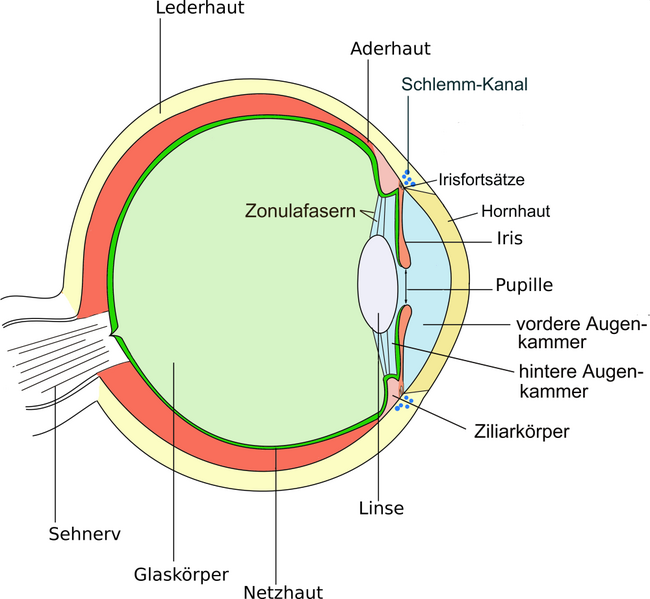
\includegraphics[width=5.4cm]{../img/Auge.png}

\paragraph{Prinzip des Sehens}
ca. 380-750nm ($4*10^{14} Hz - 7,5 * 10^{14} Hz \approx$ 1 Oktave;  $\lambda = \frac c f$); 100dB; spektr. Empf. je nach Adaption: Tagsehen / photopische Sehen / Farbempfinden bzw. Nachtsehen / scotopische Sehen; Sakkade $\Ra$ fovea centralis; 
\end{sectionbox}

\begin{sectionbox}
\subsubsection{Psychooptische und physik. Messgrößen}
1cd $\cong$ Lichtstärke eines monochromatischen strahles mit $f = 5.4 \cdot 10^{14} Hz$ und der Strahlungsstärke von $\frac{1}{683} \frac{W}{s r}$
	\begin{tablebox}{llll}
		\multicolumn{2}{c}{\emph{Psychooptik}} &\multicolumn{2}{c}{\emph{Physik}}\\
		Bezeichnung & Einheit & Bezeichnung & Einheit\\
		\cmrule
		Lichtstärke $I_v$ &$cd$ (Candela) & Strahl.stärke $I$ & $\frac{W}{sr}$\\
		Leuchtdichte $L$ & $\frac{cd}{m^2}$ & Strahl.dichte $L_{\Omega}$ & $\frac{W}{sr~m^2}$\\
		Lichtstrom $\Phi_v$ & $lm = cd~sr$ & Strahl.leistung $P$ & $W$\\
		Lichtmenge $Q_e$ & $lm\cdot s$ & Strahl.energie $E$ & $J = Ws$\\
		Beleucht.stärke $E_v$ & $lx=\frac{lm}{m^2}$ & Bestrahl.stärke $E$ & $\frac{W}{m^2}$\\
		Belichtung $H$ & $lx \cdot s$ & Energiedichte $w$ & $\frac{J}{m^2}$\\
		\cmrule
		\multicolumn{4}{c}{Lichtausbeute $\mu = \frac{Lichtstrom}{Stahlungsleistung} 1 \frac{lm}{W}$}\\
	\end{tablebox}
\end{sectionbox}
 

\begin{sectionbox}
\subsubsection{Farbsehen}
Stäbchen sw, hohe Konz($1.2 * 10^8$), Nachtsehen; S-Zapfen Blau 430nm, M-Zapfen Grün 530nm, L-Zapfen Rot 560nm, 1:10:10,  insg. $7 *10^6$; 
\end{sectionbox}

\begin{sectionbox}
\subsubsection{Gesichtsfeld}
volles Farbemfpinden nur im Überlappungsbereich der Farbzonen; primäres Gesichtsfeld horiz. $-15^\circ < \theta < + 15^\circ $ und vert. $-17^\circ < \phi < + 14 ^\circ $; 3D: $-55^\circ < \theta < 55^\circ$
\end{sectionbox}


\begin{sectionbox}
	\subsection{Farbmischung}
	\begin{tablebox}{p{\textwidth}}
		\emph{Arten der Farbmischung} \\ % topicbox
		\cmrule
		\emph{Additiv} aktive Primärstrahler; RGB; \\
		\emph{Subtraktiv} CMY ; Absorption best. Prim.farben; Ausgegangen wird von einer weiß beleuchteten Oberfläche; 
	\end{tablebox}

\paragraph{Farbwürfel}Grundfarben, Mischungen, s/w definieren Ecken; $(R,G,B)^T = (1,1,1)^T - (C,M,Y)^T$;\\ 
\end{sectionbox}
\vspace{8cm}

\columnbreak
\pagebreak 
%\includegraphics*[scale=0.6]{farbwuerfel}



\begin{sectionbox}
\subsubsection{CIE}
\parbox{3.5cm}{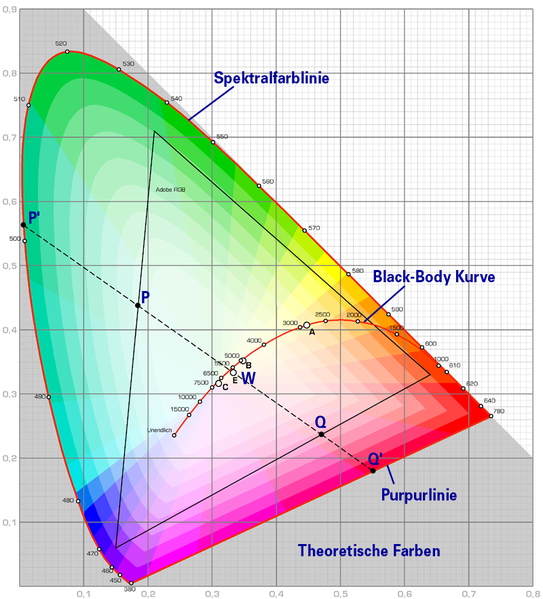
\includegraphics[width=3.5cm]{../img/CIE-Normfarbtafel.png}}
\parbox{3.3cm}{\paragraph{Normfarbtafel nach C.I.E}Ziel: Farbeindruck sämtlicher spektraler Farben duch additive Überlagerung dreie monochromatischer Strahler nachzubilden; $\lambda _{R, CIE} = 700 nm, \lambda _{G, CIE} = 546.1 nm, \lambda _{B, CIE} = 435.8 nm$ sog. Normvalenzen; \\
Im Bereich $350 nm < \lambda_R < 540 nm$ negativ; $\Ra$ nachzubildende Farbe mit rot überlagert; $\Ra$ es ist nicht möglich, alle wahrnehmbaren Farben mit nur drei Primärstrahlern nachzubilden; 
}
\paragraph{Virtuelle Normvalenzen} Uneigentliche Farbmischung; X(r), Y(g), Z(b); exist nicht real durch add. Farbmischung, können aber jede wahrnehmbare Farbe darstellen; 


\begin{equation*}
	\begin{pmatrix} 	X \\ Y \\ Z \end{pmatrix} = \overbrace{\begin{pmatrix}
	0.49 & 0.31 & 0.2 \\
	0.177 & 0.813 & 0.01 \\
	0 & 0.01 & 0.99
\end{pmatrix} }^T\begin{pmatrix}
	R_{CIE} \\ G_{CIE} \\ B_{CIE}
\end{pmatrix}
\end{equation*}

Daraus ergibt sich $z = 1 - (x+y)$; Die Farbeindrücke durch elmag Wellen best. F, befinden sich auf Begrenzunglinie der Fläche. Im Inneren befinden sich sämtliche Mischfarben, die durch Mischug der x und y Valenzen erzeugen lassen; Weißpunkt im schwerpunkt; Luminanznormierte Normkarte: 
\vspace{0.3em}

\begin{emphbox}
$x + y + z = 1$\\
$\Ra z = 1 - (x+y)$
\end{emphbox}

\vspace{0.3em}

\begin{tablebox}{lcr}
	$x = \frac{X}{X + Y + Z}$ & $y = \frac{Y}{X + Y + Z}$ & $z = \frac{Z}{X + Y + Z}$\\
\end{tablebox}
\end{sectionbox}

%\includegraphics*[scale=0.275]{luminanznormierte_normkarte}

\subsection{Hören}
%\includegraphics*[scale=0.2, angle=270]{ohr}

\begin{sectionbox}
\subsubsection{Das Ohr}
 Außenohr (Ohrmuschel \& Gehörgang); Mittelohr (Trommelfell, Gehörknöchelchen (Hammer, Amboss, Steigbügel) \& Euchstachische Röhre) - Wandlung von Luftschwingung in mech. Schwingung; Innenohr (Steigbügel über ovale Fenster in mit Flüssigkeit gefüllte Schnecke) Impedanzwandlung von Luft zu Flüssigkeit; 

Basilarmembran: Haarzellen (25k - 30k Rezeptoren) wandeln Schwingung in el. Nervenimpulse, Frequenz-Ort-Wandlung, Zerlegung in Frequenzanteile $\Ra$ Hörnerv (30k Nervenfasern) $\Ra$ Hirn
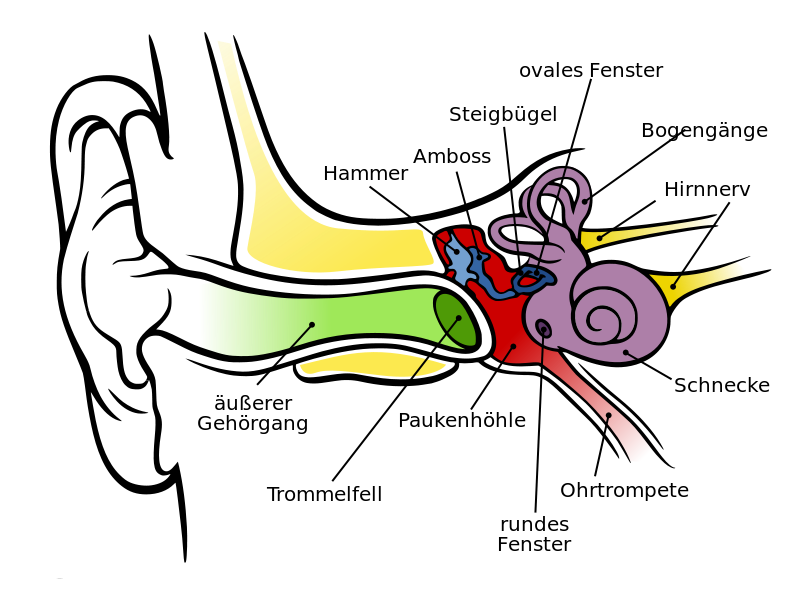
\includegraphics[width=6.5cm]{../img/Ohr.png}
\end{sectionbox}

\begin{sectionbox}
\subsubsection{Psychoakustik}
 Empfindlich von etwa 20 Hz - 20 kHz ($\approx$ 10 Oktaven); starke Dämpfung für sehr niedrige und sehr hohe Frequenzen; Resonanzfrequenz des Gehörgangs bei ca. $3 \dots 3.4 kHz$; 

Lauteinheit in [sone] 1 sone $\triangleq$ Lautheit eines 1kHz Sinustons mit 40 dB

Verhältnistonhöhe [mel] 1000 mel $\triangleq$ 1000Hz


	\begin{tablebox}{llll}
		\multicolumn{2}{c}{\emph{Psychoakustik}} &\multicolumn{2}{c}{\emph{Physik}}\\
		Bezeichnung & Einheit & Bezeichnung & Einheit\\
		\cmrule
		Tonheit $Z$ &Bark& \multirow{2}{*}{ Frequenz $f$ }& \multirow{2}{*}{$Hz$}\\
		Verhältnistonh. $V$ & Mel & & \\
		& & Schalldruck $p$ & $\frac{N}{m^2} = Pa$\\
		& & Schallschnelle $v$ & $\frac{m}{s}$\\
		& & Schallintensität $I$ & $\frac{W}{m^2} = \frac{N}{s m}$\\
		Lautstrk.pegel $L_n$ & Phon & \multirow{2}{*}{Schalldruckp. $L$} &\multirow{2}{*}{ $dB$}\\
		Lautheit $N$ & sone\\
		& & Schallleist. $P_{ak}$ & $W = \frac{N m}{s}$\\
		\cmrule
		\multicolumn{4}{c}{Bezugsschalldruck $p_0 = 2\cdot 10^{-5} \frac{N}{m^2} = 20 \mu Pa$}\\
		\multicolumn{4}{c}{Bezugsintensität $I_0 = 1.0\cdot 10^{-12} \frac{W}{m^2}$}\\
	\end{tablebox}

\paragraph{Hörfläche} Bewertungsfilter mit gleichem Lautstärkeeindruck (A, B, C, D - da nichtlinear zur Lautstärke); Lautheit Z in Sone ist angepasstes Schema; 
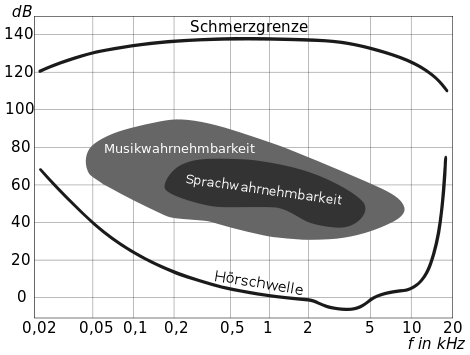
\includegraphics[width=6.5cm]{../img/Hoerflaeche.png}

\paragraph{Frequenzgruppen} (24) begrenzte Auflösung des Gehörs; jede F.gruppe nimmt gleiche Länge auf Basilarmembran ein (1,3mm - unter 500 Hz = 100Hz, drüber kleine Terz 1,19 der Mittenfrequenz); Bark-Skala; 1.31 Bark = 131 mel = 131 Hz.; Blätterrauschen in Ferne L = 10dB, Düsenjäger in 30 m L = 140dB; 

\paragraph{Verdeckungen} Hörschwelle bei Störschall (Maskierer); 

Spektrale: verbreitet sich mit steigendem Pegel überproportional; 

Zeitliche: Vorverdeckung; Simultanverdeckung; Nachverdeckung (einige hundert ms); 

Kompression: Mithörschwelle über Verdeckungen ermitteln; MP3 ab 160 kBit/s; 
\end{sectionbox}

\section{Dialogsystem}
\begin{symbolbox}
\begin{itemize}
	\item fortgeschrittene intuitive Ein-/Ausgabetechniken 
	\item Hohes Maß an Interaktivität durch Benutzerfreundlichkeit und ausgeprägte Dialogfähigkeit
	\item Intelligentes Systemverhalten, selbstständig logische Schlüsse ziehen; 
\end{itemize}
\end{symbolbox}
Teilgebiete der KI: Maschinelles Lernen, Bildverstehende Systeme, Expertensysteme, Robotik, Logik und automatisches Beweisen, Natürlichsprachliche Systeme; 

\subsection{Suchverfahren}
\begin{symbolbox}
Formulierung und Darstellung eines Problems im Zustandsraum; Graphen-Darstellung; Suchbaum;
\end{symbolbox}

\begin{emphbox}
 zyklische Wiederholungen unterbinden (gerichtete Kanten im Baum)
\end{emphbox}

\begin{sectionbox}
\subsubsection{\textcolor{darkgreen}{Tiefensuche} und \textcolor{red}{Breitensuche}}
\begin{enumerate}
	\item einelementige Liste mit Wurzelknoten
	\item bis Liste leer / Ziel erreicht: \\ -prüfe erstes Element auf Zielknoten \textcolor{darkgreen}{bzw. max. Suchtiefe} \\-wenn ja, fertig \\ - wenn nein, entferne dieses Element und füge all seine Nachfolger \textcolor{darkgreen}{ an gleicher Stelle} / \textcolor{red}{am Ende} ein.
\end{enumerate}

Vorraussetzung: Elemente der Warteliste werden systematisch erzeugt; Suchtiefe wird geeignet groß festgesetzt / ausgewertete Suchbaum muss gespeichert werden; 
\end{sectionbox}

\begin{sectionbox}
\subsubsection{Heuristische Suche / A-Algorithmus}
Verarbeitung zusätzlicher Informationen; Bewertungsmöglichkeit für Erfolgsaussichten eines bestimmten Pfades; Entscheidungen ordnen; Vielversprechende Alternative zuerst, "`dem atm billigsten folgen"'; Heuristik besteht in Definition einer geeigneten Bewertungs (Kostenfunktion) $f(n)$; z.B.

\begin{equation*}
f(n) = g(n) + h(n)
\end{equation*}

Bewertungsfunktion = Bisherige Kosten + Schätzfunktion (hier: falsche Plättchen)

Falls $h(n) \equiv 0$ gewählt wird identisch zur Breitensuche
\end{sectionbox}

\begin{sectionbox}
\subsubsection{A*-Algorithmus}
Schätzfunktion $h(n)$ monoton, d.h. Kosten werden nicht überschätzt; terminiert wenn Zielknoten gefunden und keine geringere Kostenschätzung existiert; A* somit optimaler Pfad; wird die optimale Kostenfkt $h1^*(n)$ verwendet, so wird kürzester Pfad auf Anhieb gefunden (sprich: informierte Suche); Liste mit allen Elementen erstellen + sortieren; dem insg. billigsten folgen; nix verwerfen; 
\end{sectionbox}

\section{Logik und Theorembeweisen}
\begin{sectionbox}
Wissen algorithmisch darstellen; Fakten ableiten; Behauptungen bestätigen / widerlegen; 
\end{sectionbox}

\subsection{Logik}
\begin{sectionbox}
\subsubsection{Aussagenlogik}
atomare Aussagen; wahr oder falsch; UND , ODER, NICHT; Implikation $\Rightarrow$; 
\end{sectionbox}

\begin{sectionbox}
\subsubsection{Prädikatenlogik}
Analyse und Bewertung von Beziehungen und logischen Verknüpfungen; 1. Ordnung $\Ra$ nur Veränderung von Objekten, nicht Prädikaten; Prädikate und FUnktionen, Konstanten, Variablen, Funktionen, Negation, Disjunktion, Konjunktion, Existenz-Quantor, All-Quantor, Implikation, Äquivalenz

"`In jeder Stadt gibt es einen Bürgermeister"' 
$(\forall x) \left\{ \text{Stadt}(x)  \Rightarrow (\exists y) \left[ \text{Mensch}(y) \cdot \text{Bgm}(x,y) \right] \right\}$

Regeln und Zusammenhänge aufstellen; $\Ra$ Regelwerk (Axiome); Frage (Theorem); Beweis durch Wahrheitstabelle oder Umformen der Regeln und Schlussfolgern (Resolution, Unifikation - effektiver); 
\end{sectionbox}

\begin{emphbox}
\emph{Umformregeln:}
\begin{enumerate}
	\item Doppelte Negation $\neg \neg A \equiv A$
	\item Idempotenz $ A + A \equiv A$ und $ A \cdot A \equiv A$
	\item Kommutativität $A + B \equiv B + A$
	\item Assoziativität $A + (B + C) \equiv (A + B) + C$
	\item Distributivität $A + (B \cdot C) \equiv (A + B) \cdot (A + C)$
	\item De Morgan $\neg(A \cdot B) \equiv \neg A + \neg B$
	\item Kontrapositiv $A \Rightarrow B \equiv \neg B \Rightarrow \neg A$ 
	\item $ A \Rightarrow B \equiv \neg A + B$ 
	\item $ A \Leftrightarrow B \equiv (A \Rightarrow B ) \cdot (B \Ra A) \equiv (A \cdot B) + (\neg A \cdot \neg B) $
	\item $ \neg (\forall x)A(x) \equiv (\exists x)(\neg A(x))$ 
	\item $ \neg (\exists x) A(x) \equiv (\forall x) (\neg{}A(x)) $ 
	\item $ (\forall x)(A(x) \cdot B(x)) \equiv (\forall x)A(x) \cdot (\forall y )B(y)$ 
	\item $ (\exists x)(A(x) + B(x)) \equiv (\exists x)A(x) + (\exists y)B(y)$
\end{enumerate}
\end{emphbox}

\begin{sectionbox}
\subsubsection{Standardformen}
\textcolor{red}{Konjunktive Normalform (KNF): $(A_1 + A_2 + \dots) \cdot (B_1 + B_2 + \dots) \cdot \dots$ }

Disjunktive Normalform: $(A_1 \cdot A_2 \cdot \dots) + (B_1 \cdot B_2 \cdot \dots) + \dots$

\begin{cookbox}{Regeln zur Umformung in Normalform:}
%\begin{enumerate}
	\item Eliminierung aller Äquivalenzen (\# 9)
	\item Eliminierung aller Implikationen (\# 8)
	\item Einziehung der Negation nach innen (\#6, \#10, \#11)
	\item Einführung neuer Variabeln für jeden Quantifizierer
	\item Eliminierung aller Existenz Quantoren
	\item Ausklammern der All-Quantoren und Entfallen dieser
	\item Anwendung des Distributivgesetzes zur Transofrmation in Konjunktive Normalform (\#5)
	\item Eliminierung der UND-Verknüpfungen durch Auflistung der Klauseln
	\item Einführung getrennter Variablen für jede Klausel
%\end{enumerate}
\end{cookbox}
\end{sectionbox}

\subsection{Theorembeweis}

\begin{sectionbox}
\subsubsection{Resolutionsverfahren}
Gegeben sind zwei Formel der Form: 

\begin{equation*}
\begin{split}
	A_1 + A_2 + \dots + A_n + \textcolor{red}{ P } \\
	B_1 + B_2 + \dots + B_n + \textcolor{red}{ \neg P } \\
	\text{wird zu} \\
	A_1 + \dots  + A_n + B_1 + \dots +  B_n e\equiv R
\end{split}
\end{equation*}

Anwendung beim Theorembeweis: 

Geg.: Set von $n$ existierenden und bewiesenen Axiomen $\mathcal S = \left\{S_1 \dots S_n \right\}$ ; Es gilt T zu beweisenn

Vorgehen: Erweiterung von $\mathcal S $ zu $\mathcal S^* = \left\{S_1 \dots S_n , \neg T \right\}$ Und Resolutionieren bis leere Klausel erzeugt wird. 

\textcolor{red}{Erklärung: Statt Beweis wird Unerfüllbarkeit seines Gegenteils gezeigt. }

\begin{cookbox}{Tautologie beweisen: }
	\item Wahrheit auf KNF bringen
	\item Gegenteil auf KNF bringen
	\item Zeige, dass Gegenteil \{ \} ist. 
\end{cookbox}
\end{sectionbox}

\section{Wissensrepräsentation}
\begin{symbolbox}
effizient speichern; strukturiert darstellen; Menge von Fakten, Regeln, Prozeduren, Modellen, Daten, Heuristiken; interpretierbar mit Hilfe von Repräsentationsmechanismen; 
\end{symbolbox}

\begin{sectionbox}
\subsubsection{Prädikatenlogik}
Aufteilung in Fakten und Regeln; Standardisiert durch KNF; Resolution als Inferenzmechanismus; Formulierung aufwändig und unnatürlich; zwingend Umformung in KNF;
\end{sectionbox}

\begin{sectionbox}
\subsection{Produktionsregeln}
keine Umformung in KNF; Wenn-Dann bleibt erhalten; Vorwärts- Rückwärtsverkettung als Inferenzmechanismus; Darstellung im UND/ODER-Graphen; Fakten als Blatt, Regeln als Verzweigung;
\end{sectionbox}

\begin{sectionbox}
\begin{cookbox}{Vorwärtsverkettung}
	\item Gültige Fakten einkreisen
	\item Suchen nach Regeln, in denen diese Fakten im Bedingungsteil der Regeln vorkommen
	\item Überprüfen ob Aktionsteil der Regeln eingeleitet werden kann
	\item Back to \#2
	\item Wenn keine neuen Regeln mehr feuern, überprüfen ob ein Ziel erfüllt wurde
\end{cookbox}

\begin{cookbox}{Rückwärtsverkettung}
	\item Vorgabe eines möglichen Ziels
	\item Untersuchen der Bedingungen die zum erreichen dieses Ziels erfüllt sein müssen
	\item Formulierung dieser Bedingungen als neue Teilziele, back to \# 2
	\item Falls Ziel wg. Bedingungen nicht erreicht werden kann, back to \#1 mit anderem Ziel
	\item Wurden für ein Ziel alle Bedingungen erfüllt $\Ra$ Finish
\end{cookbox}
\end{sectionbox}

\begin{sectionbox}
\subsection{Semantische Netze}
Graphische Modelle zur Darstellung von Wissen über beziehungen zw. Objekten; entsprechen etwa Fakten der Prädikatenlogik; Knoten = Objekte; Kanten = Prädikate; Verwendung bei natürlichssprachigen Systemen; keine 2 Knoten gleicher Beschriftung; Richtung der Kanten von Bedeutung; 
\end{sectionbox}

\begin{sectionbox}
\subsection{Rahmen}
Darstellung der Zerlegung von Objekten oder Situationen in ihre Bestandteile; Ähnlichkeit zu semantischen Netzen, wesentlich mächtiger und flexibler; FrameName - zentraler Knoten, Slots - Kanten, Filler - Knoten; 

1. Suchverfahren zur Ermittlung von Beziehungen; 

2. "`Rahmen-Abgleich"'; Fakten als Fragezeichen markiert; mit aktuellen Daten auffüllen; 
\end{sectionbox}


\section{Grammatiken}
\begin{symbolbox}
natürlichsprachige Systeme; Modellierung von Dialogen; 
\end{symbolbox}

\begin{sectionbox}
\subsection{Kontextfreie Grammatiken}
CFG; $ \mathcal G = \left\{ V, T, P, S \right\} $ mit Variable (Großbuchstaben), Terminale (Kleinbuchstaben), Produktionsregel ($A \rightarrow \alpha $ mit $A \in \left\{V \right\}$ und $\alpha \in \left\{ V \cup T \right\} $), Startsymbol; 
\end{sectionbox}

\begin{sectionbox}
\subsection{Chomsky-NormalForm}
CNF; Enthält nur Produktionsregeln, bei denen auf der rechten Seite nur zwei Variablen oder nur ein terminaler Ausdruck steht: 

\begin{emphbox}
	$A \rightarrow BC$ oder $A \rightarrow a$
\end{emphbox}
\end{sectionbox}

\begin{sectionbox}
\subsection{Backus-Naur-Form (BNF)}
formal exakte Definition von Programmiersprachen; Nichtterminalsymbole werden syntaktische Variablen genannt und durch $<$,$ >$ gekennzeichnet; Darst. von Wdh. durch Rekursion; 
\end{sectionbox}

\begin{sectionbox}
\subsection{EBNF}
Erweiterte BNF; Optionen [...]; abgezählte Wdh. 4*; 
\end{sectionbox}

\begin{sectionbox}
\subsection{Parsing}
Satzgenerierung: Produktionsregeln solange anwenden, bis alle Variablen V durch terminale Symbole T ersetzt sind; Parse-Tree; Ambiguitäten; 
\end{sectionbox}

\begin{sectionbox}
\subsection{Anwendung von Grammatiken in KI}
Sprache; Mustererkennung; 
\end{sectionbox}

\begin{sectionbox}
\subsection{Beispiele}
Palindrom-String:
\begin{equation*}
S \rightarrow aSa | bSb | a* | b*
\end{equation*}

Doppelte Anzahl a wie b:
\begin{equation*}
\begin{split}
	& S \rightarrow A | SA | AS | aSC | CSa | aSD | DSa | bSB | BSb \\
	& A \rightarrow Bb | Ca | Da \\
	& B \rightarrow aa \quad C \rightarrow ab \quad D \rightarrow ba \\
\end{split}
\end{equation*}

Grammatik-Grammatik:\\
S (Satz), NP (Nominalphrase), VP (Verbalphrase), PP (Päpositionalphrase), DET (Determinator, Artikel), ADJ (Adjektiv), AUX (Hilfswort), V (Verb), PRE (Präposition) und N (Nomen)
\begin{equation*}
\begin{split}
	&  \text{S} \ra \text{NP VP} | \text{VP NP}\\
	& \text{NP} \ra  \text{DET N} |  \text{ADJ N} |  \text{DET NP} |  \text{NP PP}\\
	&  \text{VP} \ra  \text{V NP} |  \text{AUX V} |  \text{V PP} |  \text{V NP} |  \text{VP PP} |  \text{AUX VP}\\
	&  \text{PP} \ra  \text{PRE NP}\\
	&  \text{DET} \ra  \text{"`der"', "`die"', "`das"',...}\\
	&  \text{ADJ} \ra  \text{"`klein"', "`groß"',...}\\
	&  \text{AUX} \ra  \text{"`wird"',...}\\
	&  \text{V} \ra  \text{"`streicheln"',...}\\
	&  \text{PRE} \ra  \text{"`in"', "`mit"',...}\\
	&  \text{N} \ra  \text{"`Junge"', "`Hund"', "`Hand"',...}\\
\end{split}
\end{equation*}
\end{sectionbox}


\section{Automatentheorie}
\begin{symbolbox}
Verarbeitung von Symbolfolgen; Modellierung von Dialogen; 
\end{symbolbox}

\subsection{Automatentypen}
\begin{sectionbox}
\subsubsection{Zustandsautomat}
Graphenform; bestimmte Anzahl von Knoten (Zustände) und Verbindungen (Transitionen); 
\begin{equation*}
Z = (S, X, T, s_0, \mathcal F )
\end{equation*}
Set mit endlicher Anzahl Zustände, x zulässiges Alphabet für die zu verarbeitende Symbolfolge X, T Transitionsfunktionen, $s_0$ Anfangszustand, $\mathcal F$ ein Set von festgelegten Endzuständen; deterministisch / nicht-d.; 
\end{sectionbox}

\begin{sectionbox}
\subsubsection{Kellerautomaten}
komplexere Grammatiken; Erweiterung mit Stack (LIFO); Transition abhängig von Stack und Eingang; Stack leer $\Ra$ Folge akzeptiert; 
\begin{equation*}
Z = (S, X, Y, T, s_0, y_0 \mathcal F )
\end{equation*}
Y - zulässiges Alphabet fürn Stack, $y_0$ Start für Stack, $\mathcal F$ leer wenn Endzustand über leeren Stack definiert ist; 
\end{sectionbox}

\section{Dialoggestaltung}
\begin{symbolbox}
Ein-/Ausgabe; Fehlerbehandlung; Fehlertoleranz; Kenntnis der Aufgabe; Benutzergruppen; 
\end{symbolbox}

\begin{sectionbox}
\subsection{Expertensysteme}
komplexes, wissensbasiertes Softwarepaket; Wissensbasis statt Datenbasis; Komponenten zur Pflege und Erweiterung dieser Basis; Schließregeln können neues Wissen produzieren; 
\end{sectionbox}

\begin{sectionbox}
\subsection{Wissen}
informelles, technisches (Algorithmen, Formeln, fixe Formeln, variable Daten), formales (wenn-dann, variable formeln + daten); 
\end{sectionbox}

\begin{sectionbox}
\subsection{Einsatzgebiete}
komplexe Aufgabenstellungen; Diagnoseaufgaben; Konfigurationsaufgaben; Beratungsaufgaben; 
\end{sectionbox}

\begin{sectionbox}
\subsection{Aufbau}
Wissensbasis: Fakten, Regeln, Prozeduren; wichtigste Komponente; 

Inferenzkomponente: Verarbeitung; Such- Verkettungsmechanismus; 

Erklärungskomponente: Lösungsweg; graphisch; Debugging; 

Dialogkomponente: Interface; 

Wissenserwerbkomponente: effiziente Entlastung des Programmierers; 

Experten, Entwickler, Anwender; 
\end{sectionbox}

\begin{sectionbox}
\subsection{Dialogformen}
Frage-Antwort; Menüauswahl; Formular; Kommandosprachen; Natürlichsprachlich; Direkte Manipulation; Multimediadialog; 
\end{sectionbox}

\section{Sprachkommunikation}
\begin{sectionbox}
eine der natürlichsten Kommunikationsformen; größtes Potential; bedeutendste \& komplexeste Teil: Spracherkennung; 
\end{sectionbox}

\begin{sectionbox}
\subsection{Klassifizierung}
Zuordnung zu Bedeutungseinheiten; Merkmalsextraktion; Merkmalsvektor; Merkmalsraum; Klassen; Training; 
\end{sectionbox}

\begin{sectionbox}
\subsection{Abstandsklassifikatoren}
Distanz eines Mustervektors zu Klasse; 

\begin{equation*}
\begin{split}
 & m_k = \frac{1}{M_k} \sum\limits^{M_k}_{i=1} r_{k,i} \\
 & d_k (x, m_k) = (x - m_k)^T * W_k * (x-m_k) \\
 & \text{Trennfunktion: } \\
 & d_1 (x, m_1) - d_2 (x, m_2) = 0
\end{split}
\end{equation*}

Gewichtsmatrix $W_k$ entscheidend; $m_k$ wird im Training ermittelt; $x$ gehört zur Klass mit min. Abstand; 

Quadratischer Abstand: $W_k$ ist Einheitsmatrix; Trennfunktion ist eine Gerade;

Mahalanobis Abstand: \textbf{Inverse} der Kovarianzmatrix; Abhängig von Klasse; Bestandteil des Trainings; Trennfunktion ist Kegelschnitt (Gerad, Ellipse, Parabel, Hyperbel)
\begin{equation*}
\begin{split}
	& W_{K,k} = \frac{1}{M_k} \sum\limits^{M_k}_{i=1} r_{k,i} \cdot r^T_{k,i} \quad -m_k \cdot m_k^T \\
	& A^{-1} = \frac{1}{ad-bc}\begin{bmatrix} d & -b \\ -c & a \end{bmatrix}
\end{split}
\end{equation*}
\end{sectionbox}

\columnbreak


\section{HMM und Algorithmen}

\begin{sectionbox}
\subsubsection{Markov-Modelle}
Abbildung stochastischer Prozesse, deren aktueller Zustand nur vom vorausgegangenen Zustand abhängt; Matrixdarstellung \begin{equation*}
A = p \left\{ q_{t+1} = s_j | q_t = s_i \right\}
\end{equation*}
Startzustand $q_1$; Vektor $e = (p(q_1 = s_1), \dots , p(q_1 = s_N))^T$ der Einsprungwahrscheinlichkeit
\end{sectionbox}

\subsection{HMM}

\begin{sectionbox}
Hidden-Markov-Modelle; statistischer Klassifikator; liefert $p$ dass eine Beobachtung einer best. Klasse zugeordnet werden kann; klassifizieren ganze Sequenzen (dynamische Folgen); "`Finde diejenige Klasse, die die Beobachtung $o=(o_1, o_2, \dots , o_t)$ am besten nachbilden kann."';  
\end{sectionbox}

\begin{sectionbox}
\subsubsection{HMM}
stochastische Version eines endlichen Zustandautomaten; Zustandsübergänge und Symbolemissionen nicht deterministisch; Beobachtungswahrscheinlichkeitsmatrix; $v = (V_1, \dots, v_M)$ Menge der möglichen Beobachtungen; 

\begin{equation*}
\begin{split}
&	B = \begin{bmatrix}
	p(v_1 | s_1) & \dots & p(v_1 | s_N) \\
	\vdots & \ddots & \vdots \\
	p(v_M | s_1) & \dots & p(V_m | s_N) \\
\end{bmatrix} \\
& \lambda = (e, A, B) \\
& p(o | \lambda ) \\
\end{split}
\end{equation*}

Von Beobachtungsfolge o kann i.A. nicht auf durchlaufene Zustandsfolge q geschlossen werden (hidden)

\begin{tablebox}{p{\textwidth}}
\emph{HMM - Eigenschaften} \\ % topicbox
\cmrule
\emph{Ergodisches HMM} \quad Es kann aus jedem Zustand in jeder andere Zustand erreicht werden; A ist voll besetzt \\
\emph{Links-Rechts-HMM} \quad keine Rücksprünge; kausal; A hat rechte obere Dreiecksform; Graphisch nach rechts aufsteigend $\Ra$ Name
\end{tablebox}
\end{sectionbox}

\begin{sectionbox}
\subsubsection{Klassifizierung mit HMM}
Pro Klasse ein HMM; das HMM welches die größte Produktionswahrscheinlichkeit $p(o|\lambda_k)$ liefert repräsentiert die gesuchte Klasse $k_x$; 
\end{sectionbox}

\begin{sectionbox}
\subsubsection{Training von HMM}
Kompensation von Störungen; Bed.: geeignete Parameter $\lambda_k$; Training mit iterativen Verfahren; $\Ra$ Baum-Welch-Algorithmus
\end{sectionbox}

\begin{sectionbox}
\subsubsection{Trellis}
Zeitabfolge in Diagramm; Berechnung sehr rechenintensiv ($OPS ~ 2T + N^T$); Weg $q$; 
\begin{equation*}
p(o | \lambda_k) = \sum\limits_{q \in Q} e_{q1} b_{q1} (o_1) \prod\limits^T _{t=2} a_{q_{t-1} q_t} b_{q_t} (o_t)
\end{equation*}
\end{sectionbox}

\subsection{HMM in der Spracherkennung}

\begin{symbolbox}
Cepstrum;  Merkmalsexrahierung; 12D Merkmalsvektor;
\end{symbolbox}

\begin{sectionbox}
\subsubsection{Modelle}
Einzelworterkenner vs. fließende Sprache; Phoneme, kleinste bedeutungsunterscheidenden Lauteinheiten; HMM pro Phonem; Pausen; 
\end{sectionbox}

\begin{sectionbox}
\subsubsection{Training}
Zusammenfassung der Phonem HMM zu einem HMM; 
\end{sectionbox}

\begin{sectionbox}
\subsubsection{Erkennung}
Wörterbücher, Grammatiken, Wahrscheinlichkeiten bestimmter Phonemkombinationen, Sprachmodelle für Wortkombinationen; 
\end{sectionbox}

\subsection{HMM-Algorithmen}
\begin{sectionbox}
\subsubsection{Vorwärts-Algorithmus}
Vorwärts-Wahrscheinlichkeit:

$\alpha_t (i) = \P(o_1, o_2, \dots , o_t , q_t = s_i | \lambda_k)$

d.h. die Wahrscheinlichkeit, dass die Teilbeobachtung $o_i$ emittiert werden und das sich das HMM zu t im Zustand $s_i$ befindet; 

\begin{cookbox}{Vorwärts-Algorithmus (Rekursiv)}
	\item Initialisierung: \\
		$\alpha_1(i) = e_i b_i (o_1), \quad 1 \leq i \leq N $\\
	\item Induktion: \\
		$ \alpha_{t+1} (j) = \left[ \sum\limits_{i=1}^N{\alpha_t (i) a_{ij}} \right] b_j (o_{t+1}) $\\
		$  \quad 1 \leq t \leq T-1; \quad 1 \leq j \leq N;$\\
	\item Terminierung \\
		$\P(o|\lambda_k )= \sum\limits_{i=1}^N \alpha _T (i)$\\
\end{cookbox}
Benötigte OPS : $T * N^2$; 
\end{sectionbox}

\begin{sectionbox}
\subsubsection{Baum-Welch-Algorithmus}
Rückwärtswahrscheinlichkeit:

 $\beta_t(i) = P(o_{t+1}, o_{t+2}, \dots , o_{T} | q_t = s_i , \lambda _k)$; 

d.h. Wahrscheinlichkeit, die restlichen Teilbeob. zu emmttieren;

\begin{cookbox}{Baum-Welch-Algorithmus (Rekursiv)}
	\item Initialisierung\\
		 $\beta_T (i) = 1 \quad 1 \leq i \leq N $\\
	\item Induktion\\
		$\beta_t(i) = \sum\limits_{j=1}^N a_{ij} b_j (o_{t+1}) \beta_{t+1} (j)$\\
		$t = T-1, T-2, \dots 1 \quad 1 \leq i \leq N$\\
\end{cookbox}

Wahrscheinlichkeit, dass sich dass HMM zu t im Zustand $s_i$ befindet und o emmitiert wird; Summe drüber $\Ra$  "`alle Aufenthalte im Zustand $s_i$"'
\begin{equation*}
\gamma _t (i) = \frac{\alpha_t (i) \beta_t (i)}{\sum \limits_{i=1}^N \alpha_t (i) \beta_t (i)}
\end{equation*}

Wahrscheinlichkeit, dass sich das HMM zu t in $s_i$ und zu t+1 in $s_j$ befindet; Summe drüber $\Ra$ "`aller Übergänge von $s_i$ zu $s_j$; 
\begin{equation*}
\begin{split}
&\xi_t (i,j) = \frac{\alpha _t (i) a_{ij} b_j (o_{t+1}) \beta_{t+1}(j)}{\sum \limits_{i=1}^N \alpha_t (i) \beta_t (i)}\\
&\gamma_t (i) = \sum\limits_{j=1}^N \xi
\end{split}
\end{equation*}

\end{sectionbox}

\begin{sectionbox}
\subsubsection{Viterbi-Algo}
meist reicht Kenntnis des wahrscheinlichsten Pfades; 
\begin{cookbox}{Viterbi-Algorithmus}
	\item Initialisierung: \\
		$\delta_1 (i) = e_i b_i (o_1) \quad 1 \leq i \leq N $\\
		$\psi _1 (i) = 0$\\
	\item Induktion: \\
		$\delta_t (j) = \max\limits_{1 \leq i \leq N }\left[ \delta_{t-1} (i) a_{ij} \right] b_j (o_t)$\\
		$\psi_t(j) = \underset{1 \leq i \leq N}{\operatorname{argmax}} \left[\delta_{t-1}(i) a_{ij} \right]$\\
		$2 \leq t \leq T; \quad 1 \leq j \leq N$\\
	\item Terminierung: \\
		$P^* = \max\limits_{1 \leq i \leq n} [\delta_t(i)]$\\
		$q_T^* = \max\limits_{1 \leq i \leq n} [\delta_t(i)]$\\
	\item Ermittlung der wahrsch. Zustandsfolge:\\
		$q_t^* = \psi_{t+1}(q^*_{t+1})$\\
		$t= T-1, T-2, \dots , 1$\\
\end{cookbox}
\end{sectionbox}


%\includegraphics*[scale=0.3]{Zapfenverteilung}

%\includegraphics*[scale=0.75]{Farbwuerfel}


%\includegraphics*[scale=0.4]{CIE_real}
%\includegraphics*[scale=0.9]{CIE_virtuell}
%\includegraphics*[scale=0.9]{CIE_Normkarte}

%\includegraphics*[scale=0.22]{Hoerflaeche}

% Dokumentende
% ======================================================================
\end{document}
